% (find-LATEX "2020-1-C3-taylor-3.tex")
% (defun c () (interactive) (find-LATEXsh "lualatex -record 2020-1-C3-taylor-3.tex" :end))
% (defun D () (interactive) (find-pdf-page      "~/LATEX/2020-1-C3-taylor-3.pdf"))
% (defun d () (interactive) (find-pdftools-page "~/LATEX/2020-1-C3-taylor-3.pdf"))
% (defun e () (interactive) (find-LATEX "2020-1-C3-taylor-3.tex"))
% (defun u () (interactive) (find-latex-upload-links "2020-1-C3-taylor-3"))
% (defun v () (interactive) (find-2a '(e) '(d)) (g))
% (find-pdf-page   "~/LATEX/2020-1-C3-taylor-3.pdf")
% (find-sh0 "cp -v  ~/LATEX/2020-1-C3-taylor-3.pdf /tmp/")
% (find-sh0 "cp -v  ~/LATEX/2020-1-C3-taylor-3.pdf /tmp/pen/")
%   file:///home/edrx/LATEX/2020-1-C3-taylor-3.pdf
%               file:///tmp/2020-1-C3-taylor-3.pdf
%           file:///tmp/pen/2020-1-C3-taylor-3.pdf
% http://angg.twu.net/LATEX/2020-1-C3-taylor-3.pdf
% (find-C3-aula-links "2020-1-C3-taylor-3" "7" "taylor3")
% (find-LATEX "2019.mk")

% «.defs»		(to "defs")
% «.title»		(to "title")
% «.na-aula-passada»	(to "na-aula-passada")
% «.na-aula-passada-2»	(to "na-aula-passada-2")
% «.exercicio-1»	(to "exercicio-1")
% «.exercicio-2»	(to "exercicio-2")
% «.exercicio-3»	(to "exercicio-3")
% «.exercicio-4»	(to "exercicio-4")
% «.exercicio-5»	(to "exercicio-5")

\documentclass[oneside,12pt]{article}
\usepackage[colorlinks,citecolor=DarkRed,urlcolor=DarkRed]{hyperref} % (find-es "tex" "hyperref")
\usepackage{amsmath}
\usepackage{amsfonts}
\usepackage{amssymb}
\usepackage{pict2e}
\usepackage[x11names,svgnames]{xcolor} % (find-es "tex" "xcolor")
%\usepackage{colorweb}                 % (find-es "tex" "colorweb")
%\usepackage{tikz}
%
% (find-dn6 "preamble6.lua" "preamble0")
%\usepackage{proof}   % For derivation trees ("%:" lines)
%\input diagxy        % For 2D diagrams ("%D" lines)
%\xyoption{curve}     % For the ".curve=" feature in 2D diagrams
%
\usepackage{edrx15}               % (find-LATEX "edrx15.sty")
\input edrxaccents.tex            % (find-LATEX "edrxaccents.tex")
\input edrxchars.tex              % (find-LATEX "edrxchars.tex")
\input edrxheadfoot.tex           % (find-LATEX "edrxheadfoot.tex")
\input edrxgac2.tex               % (find-LATEX "edrxgac2.tex")
%
%\usepackage[backend=biber,
%   style=alphabetic]{biblatex}            % (find-es "tex" "biber")
%\addbibresource{catsem-slides.bib}        % (find-LATEX "catsem-slides.bib")
%
% (find-es "tex" "geometry")
\usepackage[a6paper, landscape,
            top=1.5cm, bottom=.25cm, left=1cm, right=1cm, includefoot
           ]{geometry}
%
\begin{document}

\catcode`\^^J=10
\directlua{dofile "dednat6load.lua"}  % (find-LATEX "dednat6load.lua")

% %L dofile "edrxtikz.lua"  -- (find-LATEX "edrxtikz.lua")
% %L dofile "edrxpict.lua"  -- (find-LATEX "edrxpict.lua")
% \pu


% «defs»  (to ".defs")
% (find-LATEX "edrx15.sty" "colors-2019")
\long\def\ColorRed   #1{{\color{Red1}#1}}
\long\def\ColorViolet#1{{\color{MagentaVioletLight}#1}}
\long\def\ColorViolet#1{{\color{Violet!50!black}#1}}
\long\def\ColorGreen #1{{\color{SpringDarkHard}#1}}
\long\def\ColorGreen #1{{\color{SpringGreenDark}#1}}
\long\def\ColorGreen #1{{\color{SpringGreen4}#1}}
\long\def\ColorGray  #1{{\color{GrayLight}#1}}
\long\def\ColorGray  #1{{\color{black!30!white}#1}}
\long\def\ColorBrown #1{{\color{Brown}#1}}
\long\def\ColorBrown #1{{\color{brown}#1}}

\long\def\ColorShort #1{{\color{SpringGreen4}#1}}
\long\def\ColorLong  #1{{\color{Red1}#1}}

\def\frown{\ensuremath{{=}{(}}}
\def\True {\mathbf{V}}
\def\False{\mathbf{F}}

\def\drafturl{http://angg.twu.net/LATEX/2020-1-C2.pdf}
\def\drafturl{http://angg.twu.net/2020.1-C2.html}
\def\draftfooter{\tiny \href{\drafturl}{\jobname{}} \ColorBrown{\shorttoday{} \hours}}


%  _____ _ _   _                               
% |_   _(_) |_| | ___   _ __   __ _  __ _  ___ 
%   | | | | __| |/ _ \ | '_ \ / _` |/ _` |/ _ \
%   | | | | |_| |  __/ | |_) | (_| | (_| |  __/
%   |_| |_|\__|_|\___| | .__/ \__,_|\__, |\___|
%                      |_|          |___/      
%
% «title»  (to ".title")
% (c3m201taylor3p 1 "title")
% (c3m201taylor3a   "title")

\thispagestyle{empty}

\begin{center}

\vspace*{1.2cm}

{\bf \Large Cálculo 3 - 2020.1}

\bsk

Aulas 7 e 8: dx, $Δx$ e série de Taylor

\bsk

Eduardo Ochs - RCN/PURO/UFF

\url{http://angg.twu.net/2020.1-C3.html}

\end{center}

\newpage

% «na-aula-passada»  (to ".na-aula-passada")
% (c3m201taylor3p 2 "na-aula-passada")
% (c3m201taylor3    "na-aula-passada")

Na aula passada nós fizemos alguns exercícios pra revisar a linguagem
que o João Carlos Vieira Sampaio, da UFSCar, usou na ``Aula 14'' dele
-- que vamos tentar decifrar. Links:

\ssk

\url{https://www.dm.ufscar.br/profs/sampaio/calculo1\_aula14.pdf}

\url{http://angg.twu.net/LATEX/2020-1-C3-taylor-2.pdf}

\ssk

Nos nossos exercícios nós mantivemos as várias linguagens separadas --
veja a próxima página. Nos itens [a], [b], [c], usamos a ``notação de
Lagrange'', $f'(x)$; nos itens [a'], [b'], [c'] usamos a ``notação de
Leibniz'', $\frac{dy}{dx}$, e no item [c''] começamos a usar {\sl
  diferenciais}, como $dx$ e $dy$, que o João Carlos explica na seção
14.2 da aula dele.

\newpage

% «na-aula-passada-2»  (to ".na-aula-passada-2")
% (c3m201taylor3p 3 "na-aula-passada-2")
% (c3m201taylor3    "na-aula-passada-2")

%\printbibliography
% (find-latexinkscape-links "aula6")
% (find-latexinkscape-links "2020-1-C3/aula6_diferenciais")
% (find-pdf-page "~/LATEX/2020-1-C3/aula6_diferenciais.pdf")
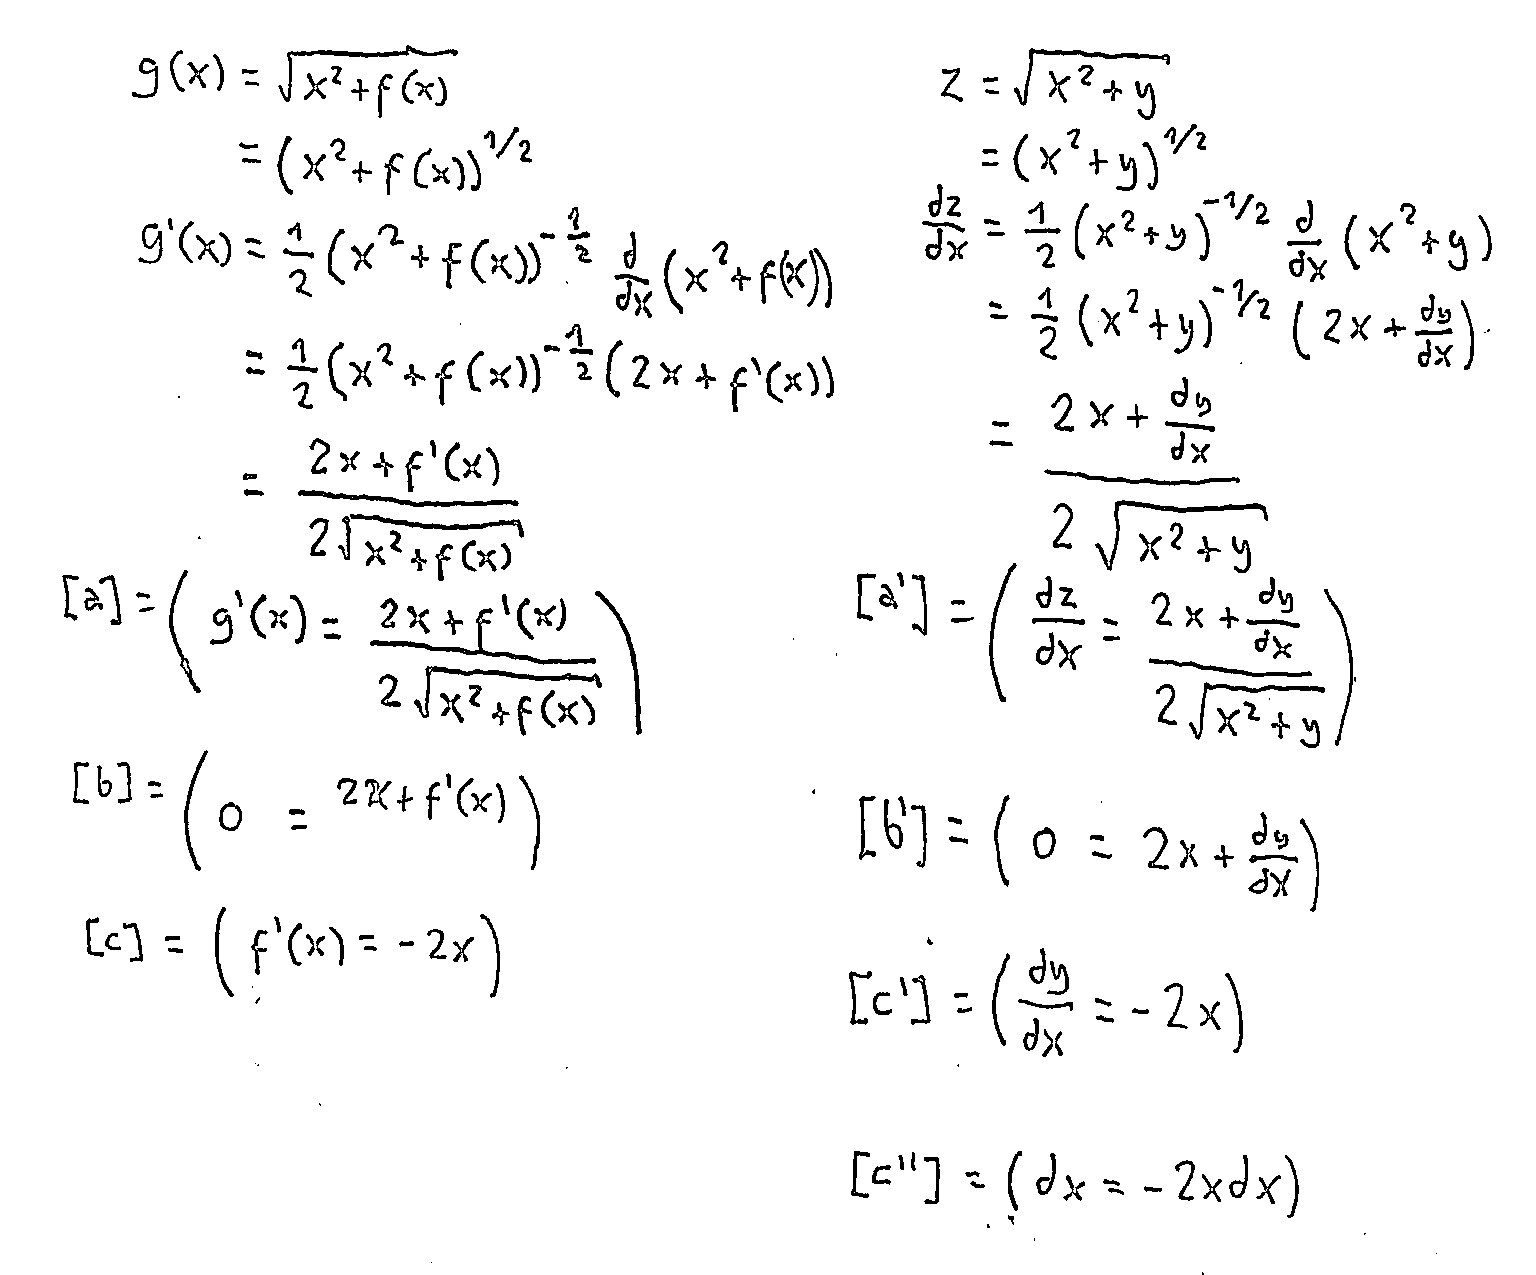
\includegraphics[height=8cm]{2020-1-C3/aula6_diferenciais.pdf}

\newpage

...mas faltou introduzirmos notações como $x_0$, $x_1$, $y_0$, $y_1$,
$Δx$, $Δy$, etc, e juntarmos tudo isto com séries de Taylor e com as
aproximações de 1ª e 2ª ordem, que em geral vamos usar na notação de
baixo...

% (c3m201taylor1p 12 "taylor-8")
% (c3m201taylor1     "taylor-8")

%
$$\begin{array}{rcl}
  f(x) &=& \displaystyle \sum_{k=0}^∞ \frac{f^{(k)}(a)}{k!} (x-a)^k \\[10pt]
  f(x) &≈& f(a) + f'(a)(x-a) \\
  f(x) &≈& f(a) + f'(a)(x-a) + \frac{f''(a)}{2} (x-a)^2 \\
  \\
  f(x_1) &=& \displaystyle \sum_{k=0}^∞ \frac{f^{(k)}(x_0)}{k!} (Δx)^k \\[10pt]
  f(x_1) &≈& f(x_0) + f'(x_0)Δx \\
  f(x_1) &≈& f(x_0) + f'(x_0)Δx + \frac{f''(x_0)}{2} Δx^2 \\
  \end{array}
$$


\newpage

% «exercicio-1»  (to ".exercicio-1")
% (c3m201taylor3p 5 "exercicio-1")
% (c3m201taylor3    "exercicio-1")

{\bf Exercício 1.}

{\sl Importante: tente fazer tudo aqui sem calculadora exceto nos
  itens que dizem ``usando a calculadora''!}

Seja $y=f(x)=\sqrt{x}$.

a) Desenhe o gráfico de $y=f(x)$ entre $x=0$ e $x=9$.

b) Digamos que $x_0=4$ e $x_1=5$. Calcule $y_0$ e $Δx$. Represente
graficamente $y_1$ e $Δy$ \ColorRed{sem calculá-los numericamente}.
Use no seu desenho as convenções da figura 14.3 do João Carlos
Sampaio.

c) Encontre uma fórmula para calcular $\frac{dy}{dx}$.

d) Calcule $\frac{dy}{dx}$ para $x=x_0$.

e) Calcule $dy$ no caso em que $x=x_0$ e $dx=Δx$.

f) Calcule $y_1$ e $Δy$ usando a calculadora.

\newpage

% «exercicio-2»  (to ".exercicio-2")
% (c3m201taylor3p 6 "exercicio-2")
% (c3m201taylor3    "exercicio-2")

A partir de uma das fórmulas de Taylor podemos obter:

$$\begin{array}{rcl}
  f(x_1)          &≈& f(x_0) + f'(x_0)Δx \\
  f(x_1) - f(x_0) &≈& f'(x_0)Δx \\
        y_1 - y_0 &≈& f'(x_0)Δx \\
               Δy &≈& \frac{dy}{dx} Δx \\
  \end{array}
$$

g) Em $f(x_1) ≈ f(x_0) + f'(x_0)Δx$ o lado esquerdo precisa de
calculadora pra ser calculado e o lado direito é uma aproximação pra
ele que pode ser calculada sem calculadora. Calcule $f(x_1)$ usando
calculadora e compare os valores dos dois lados do `$≈$'.

\bsk

{\bf Exercício 2.}

Refaça todos os itens do exercício 1 mas agora usando $x_1=1$.



\newpage

% «exercicio-3»  (to ".exercicio-3")
% (c3m201taylor3p 7 "exercicio-3")
% (c3m201taylor3    "exercicio-3")

{\bf Exercício 3.}

Nos exercícios anteriores você aprender a calcular aproximações para o
$y_1$ sem calculadora e o $y_1$ ``de verdade'' pra valores de $x_1$
dados... agora vamos generalizar isto. Seja:

$$\begin{array}{rcl}
  g(x_1) &=& f(x_0) + f'(x_0)Δx \\
         &=& f(x_0) + f'(x_0)(x_1-x_0) \\
  \end{array}
$$

a) Calcule $g(x_0)$ e $g'(x_0)$. Lembre que ainda estamos usando
$x_0=4$.

b) Represente num gráfico só as curvas $y=f(x)$ e $y=g(x)$. Obs: $g$ é
uma reta.

c) Calcule $f(0)$, $g(0)$, $f(9)$, $g(9)$, $f(-2)$, $g(-2)$. Obs: se
você souber calcular $g(0)$, $g(9)$ e $g(-2)$ só pelo gráfico sem
escrever as contas é melhor ainda.

\newpage

Dá pra fazer algo parecido pra aproximações de 2ª ordem:

$$\begin{array}{rcl}
  g(x_1) &=& f(x_0) + f'(x_0)Δx \\
         &=& f(x_0) + f'(x_0)(x_1-x_0) \\
  h(x_1) &=& f(x_0) + f'(x_0)Δx        + \frac{f''(x_0)}{2}Δx^2 \\
         &=& f(x_0) + f'(x_0)(x_1-x_0) + \frac{f''(x_0)}{2}(x_1-x_0)^2 \\
  \end{array}
$$

Vamos comparar $f(x_1)$ com $h(x_1)$ e ver que a $h(x_1)$ é uma
aproximação melhor para a $f(x_1)$ do que $g(x_1)$... mas vai ser mais
fácil visualizar isto -- e vai ser mais útil pro que vem depois -- se
usarmos trajetórias.

\newpage

% «exercicio-4»  (to ".exercicio-4")
% (c3m201taylor3p 9 "exercicio-4")
% (c3m201taylor3    "exercicio-4")

{\sl Por enquanto} as nossas fórmulas para aproximações de trajetórias
vão ser estas aqui:

$$\begin{array}{rcl}
  P(x_1) &=& (x_1,f(x_1)) \\
  Q(x_1) &=& P(x_0) + (x_1-x_0)P'(x_0) \\
  R(x_1) &=& P(x_0) + (x_1-x_0)P'(x_0) + (x_1-x_0)^2\frac{P''(x_0)}{2} \\
  \end{array}
$$

\bsk

{\bf Exercício 4.}

Nós ainda estamos usando $f(x) = \sqrt{x}$ e $x_0$ = 4.

Ainda é pra fazer tudo sem calculadora, exceto onde eu disser.

a) Represente graficamente o traço da trajetória $P$ no intervalo
$x_1∈[0,9]$ e indique os pontos $P(4)$, $P(3)$ e $P(5)$.

\newpage

{\bf Exercício 4, continuação...}
%
$$\begin{array}{rcl}
  P(x_1) &=& (x_1,f(x_1)) \\
  Q(x_1) &=& P(x_0) + (x_1-x_0)P'(x_0) \\
  R(x_1) &=& P(x_0) + (x_1-x_0)P'(x_0) + (x_1-x_0)^2\frac{P''(x_0)}{2} \\
  \end{array}
$$

b) Calcule $P(4)$, $P'(4)$ e $\frac{P''(4)}{2}$.

c) Represente graficamente os pontos $Q(4)$, $Q(3)$ e $Q(5)$. Pra
representar $Q(3)$ e $Q(5)$ \ColorRed{\bf \underline{NÃO FAÇA CONTAS}}
-- use o ponto $P(x_0)$ e o vetor $P'(x_0)$ e faça tudo direto no
gráfico.

d) Represente graficamente os pontos $R(4)$, $R(4+1)$ e $R(4-1)$. Pra
representar $R(4+1)$ e $R(4-1)$ \ColorRed{\bf \underline{NÃO FAÇA
    CONTAS}} -- use o ponto $P(x_0)$ e os vetores $P'(x_0)$ e
$\frac{P''(x_0)}{2}$ e faça tudo direto no gráfico. Depois represente
graficamente $R(4)$, $R(4+2)$ e $R(4-2)$, também sem fazer contas.

\newpage

% «exercicio-5»  (to ".exercicio-5")
% (c3m201taylor3p 11 "exercicio-5")
% (c3m201taylor3     "exercicio-5")

e) Calcule sem calculadora os valores de $Q(4.1)$ e $R(4.1)$, e depois
compare-os com o valor de $P(4.1)$ calculado usando calculadora.

\bsk
\bsk

{\bf Exercício 5}

\ssk

Refaça o exercício 3 da aula 2:

\ssk

\url{http://angg.twu.net/LATEX/2020-1-C3-vetor-tangente.pdf}

\ssk
a) Calcule $P'(t)$ e $P''(t)/2$.

b) Calcule $P(0)$, $P'(0)$ e $P''(0)/2$.

c) Calcule $P(\frac{\pi}{2})$, $P'(\frac{\pi}{2})$ e $P''(\frac{\pi}{2})/2$.

\newpage



d) Usando a fórmula
%
$$R(x_0+Δx) = P(x_0) + P'(x_0)Δx + \frac{P''(x_0)}{2}Δx^2
$$
%
com $x_0=\frac{π}{2}$, represente graficamente os pontos $R(x_0+0)$,
$R(x_0+1)$, $R(x_0-1)$, $R(x_0+2)$, $R(x_0-2)$. Tente fazer o mínimo
possível de contas --- dá pra representar esses pontos direto no
gráfico já que você já sabe $P(\frac{\pi}{2})$, $P'(\frac{\pi}{2})$ e
$P''(\frac{\pi}{2})/2$.

\ssk

e) Usando $x_0=\frac{π}{2}$ na fórmula acima calcule sem calculadora
$R(x_0+0.1)$ e depois compare o seu resultado com o resultado de
$P(x_0+0.1)$ calculado com calculadora.


% (c3m201vtp 6 "exercicio-3")
% (c3m201vt    "exercicio-3")


% (c3m201taylor2p 4 "sampaio")
% (c3m201taylor2    "sampaio")
% https://www.dm.ufscar.br/profs/sampaio/calculo1_aula14.pdf
% (code-pdf-page "sampaio14" "$S/https/www.dm.ufscar.br/profs/sampaio/calculo1_aula14.pdf")
% (code-pdf-text "sampaio14" "$S/https/www.dm.ufscar.br/profs/sampaio/calculo1_aula14.pdf")
% (find-sampaio14page)
% (find-sampaio14text)
% (find-sampaio14page 3 "14.2      Diferenciais")
% (find-sampaio14text 3 "14.2      Diferenciais")




% https://en.wikipedia.org/wiki/Leibniz%27s_notation




\end{document}

%  __  __       _        
% |  \/  | __ _| | _____ 
% | |\/| |/ _` | |/ / _ \
% | |  | | (_| |   <  __/
% |_|  |_|\__,_|_|\_\___|
%                        
% <make>

 (eepitch-shell)
 (eepitch-kill)
 (eepitch-shell)
# (find-LATEXfile "2019planar-has-1.mk")
make -f 2019.mk STEM=2020-1-C3-taylor-3 veryclean
make -f 2019.mk STEM=2020-1-C3-taylor-3 pdf

% Local Variables:
% coding: utf-8-unix
% ee-tla: "c3m201taylor3"
% End:
